%-------------Preamble-------------%
\documentclass[12 pt]{article}
\usepackage{mathptmx}
\usepackage{newtxtext,newtxmath}
\usepackage{authblk}
\usepackage{tgbonum}
\usepackage{graphicx}
\usepackage{tcolorbox}
\usepackage[spanish]{babel}
\usepackage[T1]{fontenc}
\usepackage[utf8]{inputenc}
\usepackage{listings}
\usepackage{inconsolata}
\usepackage{color}
\usepackage{xcolor}
\usepackage{pdfpages}
\usepackage{hyperref}

\renewcommand{\lstlistingname}{File}% Listing -> File

\definecolor{codegreen}{rgb}{0,0.6,0}
\definecolor{codegray}{rgb}{0.5,0.5,0.5}
\definecolor{codepurple}{rgb}{0.58,0,0.82}
\definecolor{backcolour}{rgb}{0.95,0.95,0.92}

%-----------Front Matter-----------%
\begin{document}
\setcounter{page}{1}			   % Start on page 1.
\pagenumbering{roman}			   % Roman numerals for the front matter.

%------------Front page------------%
\thispagestyle{empty}			   % Clear canvas allows for a fully customisable front page.
\begin{center}
	\noindent Universidad de Murcia\\
	\noindent INGENIERÍA INFORMÁTICA\\[0.8in]
\end{center}
\begin{figure}[h]
	\centering
	
\includegraphics[height=6 cm]{images/uni.png} % Use vectorised images whenever possible (Formats: .eps, .ps, .pdf). Exceptions are heat maps and scatter plots where it's preferable to use .png or .bmp. NEVER use .jpg, it's tacky and this is your thesis (i.e. your baby, don't feed it junk).
	\vspace{0cm}
\end{figure}
\vspace{1cm}
\begin{center}
	TECNOLOGÍAS ESPECÍFICAS DE LA INGENIERÍA INFORMÁTICA\\
	Boletín de prácticas de los bloques 3 y 4\\[1cm]
	\vfill
	{\fontfamily{lmr}\selectfont
     Autor: Victorio J. Molina Bermejo\\
	 DNI: 48632380-F \hspace{8pt} Grupo: 3.2\\
	 }
	\vfill
	\noindent FACULTAD DE INFORMÁTICA \hfill Junio 2020\\
\end{center}
\newpage
\tableofcontents
\newpage
\section{Especificación de la práctica}
Imaginemos que dada, una lista de elementos, queremos obtener una nueva versión de la misma sin
repeticiones. Python nos ofrece los conjuntos para ello, pero también podríamos conseguir lo mismo
usando listas, diccionarios, etc. Queremos evaluar las distintas posibilidades que tenemos en Python
para saber cuál es la más eficiente y compararlas con una implementación propia en C de una función
de eliminación de duplicados. Para ello, debemos implementar un programa de Python que reciba tres
parámetros: un fichero de entrada con una lista de elementos, uno por línea, un fichero de salida donde
se guardará esa misma lista de elementos, pero sin repeticiones, y un fichero de salida donde se guardará en PDF la gráfica que mostrará el tiempo usado por cada técnica para distintos tamaños de datos; esta gráfica se generará usando Matplotlib. Un detalle a tener en cuenta es que el orden de los elementos en el fichero de salida puede ser distinto de aquel que tienen en el fichero de entrada.\\

Podemos suponer que los elementos del fichero de entrada son números naturales entre 0 y un cierto
límite. Para hacer las pruebas, se recomienda generar un fichero que contenga 200000 números naturales
aleatorios entre 0 y 99999 (ambos inclusive) y hacer un estudio de cada técnica con los primeros 2000
elementos del fichero, los primeros 4000 elementos del fichero, los primeros 6000 elementos del fichero, y
así sucesivamente hasta el total de 200000 elementos. Para generar el fichero de entrada, se sugiere hacer
un pequeño programa en Python que reciba como parámetro el nombre del fichero y, usando Numpy, se
generen los 200000 números naturales entre 0 y 99999 (el número de elementos a generar también podría
ser un parámetro de entrada).\\

Al menos, hay que analizar dos formas de obtener una lista sin repeticiones usando dos estructuras de
datos distintas de Python y una tercera forma que debemos implementar en código en C y que usaremos
desde Python a través de ctypes. En esta tercera forma, la función de C a implementar debe recibir la lista de elementos original y devolver la lista de elementos sin duplicados. La memoria dinámica que sea
necesaria reservar para el intercambio de información entre el código de Python y el de C se reservará
desde Python. Los alumnos tienen que decidir qué código de C implementar para obtener el resultado
deseado de la forma más eficiente posible.\\
\newpage
Además de la gráfica generada en PDF, que habrá que incluir en el documento LATEX final donde se
explique el trabajo realizado, también habrá que incluir el resultado del perfilado (profiling) del tiempo
de ejecución de cada técnica de eliminación de duplicados usada y una gráfica que muestre el consumo de
memoria por parte del programa durante su ejecución. Para realizar estos perfilados, pueden usarse los
módulos \emph{line\_profiler} y \emph{memory\_profiler} descritos en teoría. En el perfilado del tiempo de ejecución
no es necesario hacer un estudio para cada posible tamañoo de la lista de elementos de la que hay que
eliminar duplicados. Basta con que el perfilado se haga de tal manera que refleje lo mismo que la gráfica
generada en PDF en cuanto al orden de las distintas técnicas en lo que a eficiencia se refiere.

\section{Resolución de la práctica}
\subsection{Código}
\subsubsection{Código Python}
A continuación se presenta el código Python utilizado para resolver el enunciado, desde el módulo main, y el fichero contenedor de las funciones de eliminación de duplicados, en la que se incluye el Wrapper que permite usar la biblioteca C existente, hasta el script para la generación del fichero de entrada. 

\hfill
\begin{lstlisting}[
    language=Python,
    caption=main.py,
    backgroundcolor=\color{backcolour},   
    commentstyle=\color{codegreen},
    keywordstyle=\color{magenta},
    numberstyle=\tiny\color{codegray},
    stringstyle=\color{codepurple},
    basicstyle=\ttfamily\footnotesize,
    breakatwhitespace=false,         
    breaklines=true,                 
    captionpos=b,                    
    keepspaces=true,                 
    numbers=left,                    
    numbersep=5pt,                  
    showspaces=false,                
    showstringspaces=false,
    showtabs=false,                  
    tabsize=2
]
#!/usr/bin/env python3
# -*- coding: utf-8 -*-

'''
Created on Thu May  7 01:40:07 2020

@author: VictorioMolina
'''

import sys
import utils
import matplotlib.pyplot as plt
import numpy as np
import time
from inspect import getmembers, isfunction
from matplotlib.backends.backend_pdf import PdfPages
from matplotlib import gridspec

plt.rcParams.update({'font.size': 14})
plt.rcParams.update({'figure.max_open_warning': 0})


# Method that turns the file lines into a list
def file_to_list(path):
    try:
        infile = open(path, 'r')
    except IOError:
        # The file doesn't exist
        print("The file {} doesn't exists".format(path))
        sys.exit(-1)
    else:
        # The file exists
        elements = []
        
        # Add the file lines to the list of elements
        elements.extend(int(line) for line in infile)

        infile.close()
        return elements

# Method that writes the result of the program in an specific file
def result_to_file(result, path):
    try:
        outfile = open(path, 'x')
    except FileExistsError:
        print("The file {} already exists".format(sys.argv[2]))
        sys.exit(-1)
    else:
        for element in result:
            outfile.write(str(element) + '\n')
        outfile.close()

# Method that generates a plot and save it in an specific PDF file
def generate_plots(title, x, y, pdf):
    fig = plt.figure(figsize=(14, 19.8)) # A4 Size

    fig.suptitle(title, fontsize=30)

    spec = gridspec.GridSpec(ncols=3, nrows=2, width_ratios=[0.5,4,0.5])

    # Bar plot
    ax = fig.add_subplot(spec[1])
    plt.xlabel("Execution Time")
    width = 0.75 # Bars' width
    ind = np.arange(len(y))
    ax.barh(ind, y, width, color="blue")
    ax.set_yticks(ind + width / 4)
    ax.set_yticklabels(x, minor=False)

    # Pie chart
    ax1 = fig.add_subplot(spec[4])
    explode = (0, 0, 0, 0, 0, 0.05)  # only "explode" the 6th slice which represents the C function
    ax1.pie(
        [_ * 1000 for _ in y],
        explode=explode,
        labels=x,
        autopct='%1.1f%%',
        shadow=False,
        startangle=90
    )
    ax1.axis('equal')  # Equal aspect ratio ensures that pie is drawn as a circle.

    # Save current figures in a pdf page
    pdf.savefig()



# Method that studies the efficiency of each technique for different data sizes
# generating graphics that will be saved in a pdf
def study_techniques_efficiency(seq, path):
    try:
        pdf_outfile = open(path, 'x')
    except FileExistsError:
        print("The file {} already exists".format(path))
        sys.exit(-1)
    else:
        # Create a multipage PDF file
        pdf = PdfPages(path)

        # Get all the functions of the module
        functions_list = [o for o in getmembers(utils, isfunction)]
        
        # Make an study of each technique in size intervals of 2000 elements
        size_interval = 2000
        for i in range(int(len(seq) / size_interval)):
            # For each technique, calling its function with the corresponding time taking
            cutten_list = seq[0:(i+1)*size_interval]
            exec_times = [] # Will store the exec time of each function 

            for function_name, function_obj in functions_list:
                # Calculate the exec time
                t0 = time.time_ns()
                result = function_obj(cutten_list)
                t_exec = (time.time_ns() - t0) / 1.0e9

                # Store the ecex time
                exec_times.append(t_exec)
                print("{} has taken {} seconds to execute".format(function_name, t_exec))

            # Generate a plot with the execution time stats
            generate_plots(
                    "TIMES FOR THE FIRST {} NUMBERS".format((i+1)*size_interval),
                    [f[0] for f in functions_list],
                    exec_times,
                    pdf
            )
        
        # Close the pdf
        pdf.close()

def main():
    """
        ---------------------------------------------------------------------------
        PROGRAM ARGUMENTS:
            -> infile: input file with a list of elements, one per line
            -> outfile: output file where that same list of elements will be saved, 
                    but without repetitions
            -> pdf_outfile: output file where the graph that will show the time used
                    by each technique for different data sizes will be saved in pdf
        ---------------------------------------------------------------------------

    """

    # Command line argument control
    if len(sys.argv) != 4:
        print("Usage: {} infile outfile pdf_outfile".format(sys.argv[0]))
        sys.exit(0)

    # Reading the sequence of the input file
    seq = file_to_list(sys.argv[1])

    # Calling the external function through its wrapper
    result = utils.remove_duplicates_6(seq)

    # Writing the result in the outfile
    result_to_file(result, sys.argv[2])

    # Finally, study the different techniques efficiency
    study_techniques_efficiency(seq, sys.argv[3])

if __name__ == '__main__':
    main()

\end{lstlisting}
\newpage
\begin{lstlisting}[
    language=Python,
    caption=/src/Python/utils.py,
    backgroundcolor=\color{backcolour},   
    commentstyle=\color{codegreen},
    keywordstyle=\color{magenta},
    numberstyle=\tiny\color{codegray},
    stringstyle=\color{codepurple},
    basicstyle=\ttfamily\footnotesize,
    breakatwhitespace=false,         
    breaklines=true,                 
    captionpos=b,                    
    keepspaces=true,                 
    numbers=left,                    
    numbersep=5pt,                  
    showspaces=false,                
    showstringspaces=false,
    showtabs=false,                  
    tabsize=2
]
# -*- coding: utf-8 -*-

'''
This file contains a number of useful functions for removing duplicates.

@author: VictorioMolina
'''

import ctypes, os
from functools import reduce
import numpy as np
import time


# Loading the shared library into ctypes
LIBREMOVE_DUPLICATES = ctypes.CDLL(
    os.path.abspath(
        os.path.join(os.path.dirname(__file__), "../C/libremove_duplicates.so.1")
    )
)

# @profile
def remove_duplicates_1(seq):
    # Not preserving the order
    return list(set(seq))

# @profile
def remove_duplicates_2(seq):
    # Preserving the order
    found = set()
    return [x for x in seq if not (x in found or found.add(x))]

# @profile
def remove_duplicates_3(seq):
    # Not preserving the order
    keys = {}
    for x in seq:
        keys[x] = 1
    return list(keys.keys())

# @profile
def remove_duplicates_4(seq):
    # Not preserving the order and using NumPy
    return list(np.unique(seq))

# @profile
def remove_duplicates_5(seq):
    # Preserving the order and using NumPy
    indexes = sorted(np.unique(seq, return_index=True)[1])
    return [seq[i] for i in indexes]

# Python Wrapper for calling the C function
# @profile
def remove_duplicates_6(seq):    
    # Object corresponding to the function within the library
    func_remove_duplicates = LIBREMOVE_DUPLICATES.remove_duplicates
    
    # Function protoype
    func_remove_duplicates.argtypes = [
        ctypes.POINTER(ctypes.c_uint),
        ctypes.POINTER(ctypes.c_uint),
        ctypes.c_uint
    ]
    
    # This function returns void
    func_remove_duplicates.restype = None

    # Variable in which we will collect the result of the function.   
    result = (ctypes.c_uint * len(seq))()
    
    # Call to the shared library function.
    func_remove_duplicates((ctypes.c_uint * len(seq))(*seq), result, len(seq))
    
    # Copying result of the function to another vector
    vout=[*result]  # This type of copy is the 'fastest' in Python
        
    # Removing all zeros least the first one
    while len(vout) > 1 and vout[-1] == 0:
        vout.pop()
        
    # Finally, we return the output vector
    return vout

\end{lstlisting}
\newpage
\begin{lstlisting}[
    language=Python,
    caption=/test/generate\_test\_file.py,
    backgroundcolor=\color{backcolour},   
    commentstyle=\color{codegreen},
    keywordstyle=\color{magenta},
    numberstyle=\tiny\color{codegray},
    stringstyle=\color{codepurple},
    basicstyle=\ttfamily\footnotesize,
    breakatwhitespace=false,         
    breaklines=true,                 
    captionpos=b,                    
    keepspaces=true,                 
    numbers=left,                    
    numbersep=5pt,                  
    showspaces=false,                
    showstringspaces=false,
    showtabs=false,                  
    tabsize=2
]
# Generate a file made up of random integers

import numpy as np

quantity = int(input("How many? "))
limit = int(input("Max integer: "))
filename = "numbers.txt"

numbers = np.random.randint(low=0, high=limit+1, size=quantity)

f = open(filename, 'w')
for n in numbers:
    f.write("{}\n".format(n))

\end{lstlisting}

\subsubsection{Código C}
En lo que al código C respecta, he implementado un fichero de cabecera con los prototipos de función, un fichero .c con la implementación del método de eliminación de duplicados dando uso del algoritmo \emph{Heap Sort}, además de generar un archivo Makefile para la compilación del código con la biblioteca gcc, que conlleva a la creación de la biblioteca compartida nativa de Linux \emph{libremove\_duplicates.so.1.0.1} utilizada en el wrapper de Python.

\hfill
\begin{lstlisting}[
    language=C,
    caption=/src/C/remove\_duplicates.h,
    backgroundcolor=\color{backcolour},   
    commentstyle=\color{codegreen},
    keywordstyle=\color{magenta},
    numberstyle=\tiny\color{codegray},
    stringstyle=\color{codepurple},
    basicstyle=\ttfamily\footnotesize,
    breakatwhitespace=false,         
    breaklines=true,                 
    captionpos=b,                    
    keepspaces=true,                 
    numbers=left,                    
    numbersep=5pt,                  
    showspaces=false,                
    showstringspaces=false,
    showtabs=false,                  
    tabsize=2
]
#ifndef __REMOVE_DUPLICATES_H__
#define __REMOVE_DUPLICATES_H__

/* Working with memory already reserved by Python! */

// Function Prototypes

void remove_duplicates(const unsigned int *vin,
                       unsigned int *vout,
                       const unsigned int size);               

void heap_sort(unsigned int arr[], const unsigned int size);

void create_max_heap(unsigned int arr[], 
                     const unsigned int size,
                     unsigned int root_index);
                     
void swap_nodes(unsigned int *ptr1, unsigned int *ptr2); 

#endif
\end{lstlisting}
\hfill
\begin{lstlisting}[
    language=C,
    caption=/src/C/remove\_duplicates.c,
    backgroundcolor=\color{backcolour},   
    commentstyle=\color{codegreen},
    keywordstyle=\color{magenta},
    numberstyle=\tiny\color{codegray},
    stringstyle=\color{codepurple},
    basicstyle=\ttfamily\footnotesize,
    breakatwhitespace=false,         
    breaklines=true,                 
    captionpos=b,                    
    keepspaces=true,                 
    numbers=left,                    
    numbersep=5pt,                  
    showspaces=false,                
    showstringspaces=false,
    showtabs=false,                  
    tabsize=2
]
#include "remove_duplicates.h"

// Function to remove duplicated elements in an array
void remove_duplicates(const unsigned int *vin, unsigned int *vout, const unsigned int size)
{
    /*
    
        Complexity Analysis
        ---------------------------------------------
        TIME                     O(n * log(n)) + O(n) = O(n * log(n))
        SPACE                    O(n) + O(1) = O(n)
        ---------------------------------------------
        
    */    
    
    // Creating copy of the entry vector... (good choice)
    unsigned int arr[size];
    for(int i = 0; i < size; i++)
    {
        arr[i] = vin[i];
    }
    
    // Sorting the array with the heap-sort algorithm
    heap_sort(arr, size);
    
    int i = 0;
    int j = 0;
    while (i < size)
    {
        // Insert element to the result vector
        vout[j] = arr[i];
        j = j + 1;
        
        while (arr[i] == arr[i + 1])
        {
            i = i + 1;
        }  
        i = i + 1;
    }
}

// Heap-sort main function
void heap_sort(unsigned int arr[], const unsigned int size)
{
    /*
    
        Complexity Analysis
        ---------------------------------------------
        best, worst, average TIME      O(n * log(n))
        SPACE                          O(1)
        ---------------------------------------------
        
    */
    
    for (signed int i = size / 2 - 1; i >= 0; i--)
    {
        create_max_heap(arr, size, i); 
    }
        
    for (signed int i = size - 1; i > 0; i--) 
    { 
        swap_nodes(&arr[0], &arr[i]); 
        create_max_heap(arr, i, 0);
    } 
}

// Heap-sort helper function
void create_max_heap(unsigned int arr[], const unsigned int size, unsigned int root_index)
{
    unsigned int root = root_index;
    unsigned int left = 2 * root_index + 1;
    unsigned int right = 2 * root_index + 2;
    
    // If the left son is greater than the root
    if (left < size && arr[left] > arr[root])
    {
        root = left;
    }
    
    // If the right son is greater than the root
    if (right < size && arr[right] > arr[root])
    {
        root = right;
    }
    
    // If the root has changed
    if (root != root_index)
    {
        swap_nodes(&arr[root_index], &arr[root]);
        
        // Continue resolving the new tree
        create_max_heap(arr,  size, root);
    }
}

// Heap-sort helper function
void swap_nodes(unsigned int *ptr1, unsigned int *ptr2)
{
    unsigned int tmp = *ptr1;
    *ptr1 = *ptr2;
    *ptr2 = tmp;
}

\end{lstlisting}
\hfill
\begin{lstlisting}[
    language=C,
    caption=/src/C/Makefile,
    backgroundcolor=\color{backcolour},   
    commentstyle=\color{codegreen},
    keywordstyle=\color{magenta},
    numberstyle=\tiny\color{codegray},
    stringstyle=\color{codepurple},
    basicstyle=\ttfamily\footnotesize,
    breakatwhitespace=false,         
    breaklines=true,                 
    captionpos=b,                    
    keepspaces=true,                 
    numbers=left,                    
    numbersep=5pt,                  
    showspaces=false,                
    showstringspaces=false,
    showtabs=false,                  
    tabsize=2
]
all: libremove_duplicates.so.1.0.1 libremove_duplicates.so.1

libremove_duplicates.so.1.0.1: remove_duplicates.c remove_duplicates.h
	gcc -Wall -c -fPIC -g remove_duplicates.c
	gcc -shared -Wl,-soname,libremove_duplicates.so.1 -o libremove_duplicates.so.1.0.1 remove_duplicates.o

libremove_duplicates.so.1: libremove_duplicates.so.1.0.1
	ln -s libremove_duplicates.so.1.0.1 libremove_duplicates.so.1

clean:
	rm -fr libremove_duplicates.so.1.0.1 libremove_duplicates.so.1 remove_duplicates.o *~ 
\end{lstlisting}
\newpage
\section{Guía para la ejecución del programa}
Para la ejecución del programa basta con teclear siguiente comando en el terminal:
\begin{center}
    \texttt{python3 main.py infile outfile pdf\_outfile}
\end{center}
Siendo \emph{infile} el fichero de entrada que contiene el listado de números; \emph{outfile} la ruta del fichero (inexistente) en el que se guardará el resultado del programa, es decir, la lista de numeros del fichero de entrada pero sin duplicados; y \emph{pdf\_outfile} la ruta del fichero (también inexistente) en el que se guardarán las gráficas estadísticas creadas durante el estudio de los tiempo de ejecución de las distintas técnicas de eliminación de duplicados implementadas en el programa.\\

Cabe destacar que he usado en el módulo main he usado \emph{\#!/usr/bin/env python3} para la portabilidad en diferentes sistemas en caso de que tengan el intérprete de idiomas instalado en diferentes ubicaciones, lo cual además nos permite ejecutar el programa de la siguiente manera:\\

\begin{center}
    \texttt{./main.py infile outfile pdf\_outfile}
\end{center}

\section{Herramientas utilizadas durante el desarrollo}
\subsubsection{Numpy}
Numpy es el paquete fundamental para la computación científica con Python. Entre otras cosas contiene:\\

\begin{itemize}
	\item Un poderoso objeto de matriz N-dimensional
	\item Funciones sofisticadas de broadcasting, que permite trabajar con arrays de diferentes tamaños
	\item Herramientas para integrar código C/C++
	\item Álgebra lineal útil, transformación de Fourier, y capacidades para la generación de números aleatorios
\end{itemize}

Además, una gran cantidad de paquetes de cómputo científico se apoyan de Numpy como biblioteca básica, siendo Matplotlib, biblioteca de la que hablaré en la siguiente sección, una de ellas.\\

En mi caso, me ha sido de utilidad en la eliminación de duplicados, apoyandome en las técnicas que proporciona Numpy, y la generación de numeros aleatorios.
\subsubsection{Matplotlib}
Matplotlib es el estándar de facto para realizar todo tipo de gráficos en Python, y por tanto resulta obvio que, dada la capcidad de configuración y la calidad de resultados que esta nos ofrece, durante el estudio de los tiempos de ejecución, para la generación de las gráficas para los distintos tamaños de datos, la haya utilizado.\\

He optado por "plotear" la información en gráficos de barras, ya que es la mejor opción para entender visualmente, de manera clara y sencilla, la comparativa de tiempos, y de tarta, para representar el porcentaje del tiempo total que utiliza cada técnica.\\

También he importado \emph{PdfPages} de \emph{matplotlib.backends.backend\_pdf} para crear el pdf en el que guardar todos los gráficos obtenidos.

\subsubsection{Ctypes}
Ctypes permite usar bibliotecas existentes (programadas con otros lenguajes) escribiendo simples wrappers de código en Python. Básicamente sirve como puente o interfaz entre el código Python y el código C, pues nos proporciona el mecanismo para realizar la llamada a la función C, mediante sus propios tipos de datos.\\

Antes de realizar la llamada debemos indicar el prototipo de la función externa (a la que se va invocar) mediante los atributos \emph{argtypes} y \emph{restype}.

\newpage 

\subsubsection{Profiling}
En ingeniería de software el análisis de rendimiento, comúnmenete llamado profiling, es la investigación del comportamiento de un programa usando información reunida desde el análisis dinámico del mismo. Esta técnica nos permite conocer el consumo de memoria de un programa, frecuencia y duración de las llamadas a funciones... ayudándonos a optimizarlo en algunos aspectos.\\

El profiling del tiempo de ejecución lo he realizado con el módulo \emph{line\_profiler}, mientras que el de la memoria lo he hecho con \emph{memory\_profiler}.\\

En la jerarquía de directorios del programa, concretamente en el directorio \emph{/doc/profiling} encontramos los distintos ficheros (visualizables) \texttt{main.py.lprof} y \texttt{mprofile\_20200519085312.dat} que contienen el resultado del análisis del tiempo y memoria utilizada, respectivamente.
\subsubsection{Git}
Como muchas de las grandes cosas en esta vida, Git comenzó con un poco de destrucción creativa y una gran polémica.\\

En el 2005, la relación entre la comunidad que desarrollaba el kernel de Linux y la compañía que desarrollaba BitKeeper se vino abajo y la herramienta dejó de ser ofrecida de manera gratuita. Esto impulsó a la comunidad de desarrollo de Linux (y en particular a Linus Torvalds, el creador de Linux) a desarrollar su propia herramienta basada en algunas de las lecciones que aprendieron mientras usaban BitKeeper.\\

Para el control de versiones del proyecto he utilizado esta herramienta, pues me ha permitido manipular y gestionar el código en la línea de tiempo, reflejando los distintos cambios realizados. Además cuenta con una versión gráfica llamada gitg, en la que he podido ir apreciando con los ojos los estados de las ramas que he ido creando.\\

En la siguiente figura muestro el esato final del proyecto, justo antes de importar este propio fichero Latex en la carpeta de documentación.\\

\begin{figure}[htp]
    \centering
    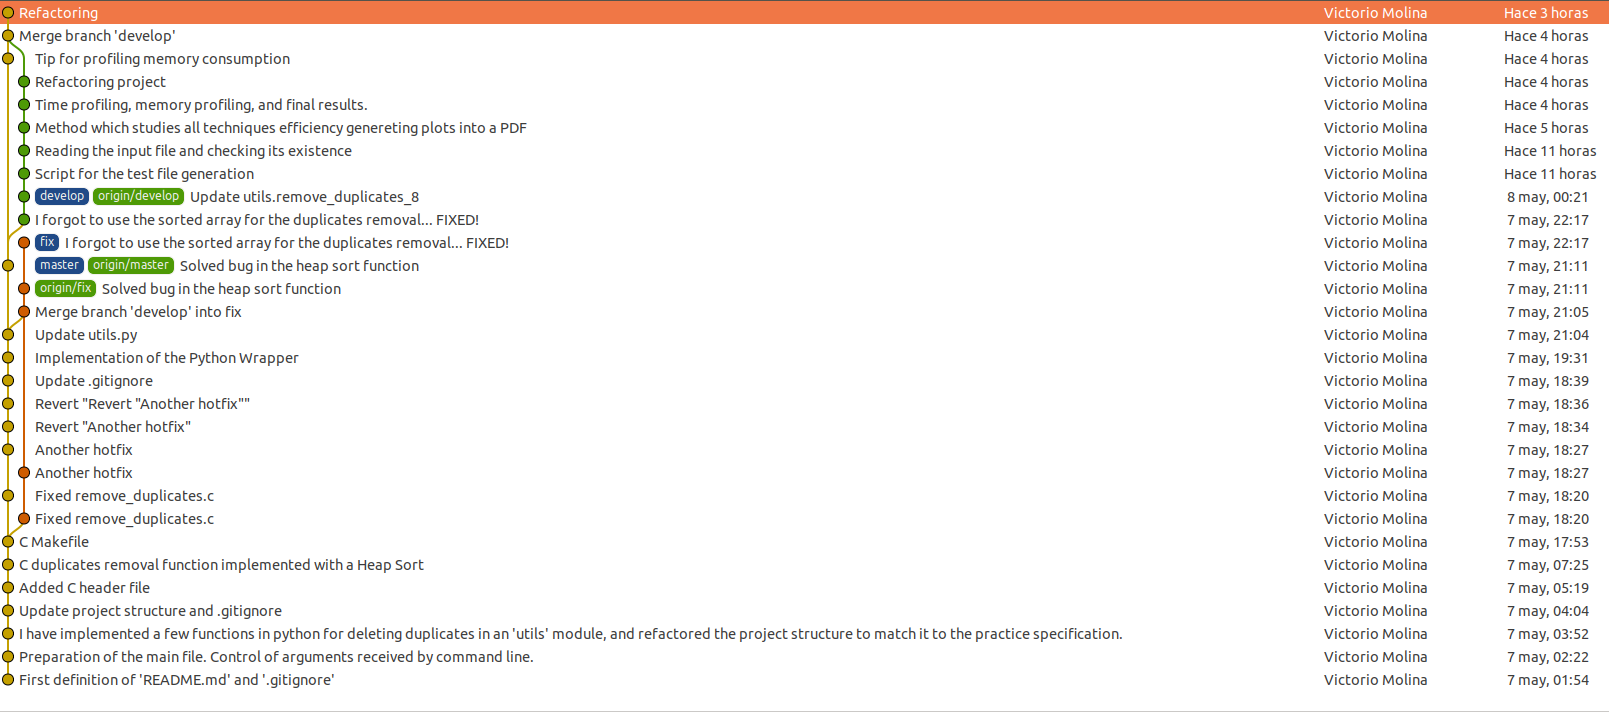
\includegraphics[width=15cm]{images/gitg.png}
    \caption{Estado final del proyecto git}
    \label{fig:gitg}
\end{figure}

\subsubsection{GitHub}
He subido el proyecto a mi repositorio online de GitHub. Este es el enlace al mismo: \href{https://github.com/VictorioMolina/Python-remove-duplicates-profiling}{https://github.com/VictorioMolina/Python-remove-duplicates-profiling}

\section{Análisis del orden de complejidad de la función C}

El algoritmo de eliminación de duplicados que he implementado es sencillo, primero ordenamos el vector de entrada (para así poder eliminar los duplicados de una pasada) mediante uno de los mejores algoritmos de ordenación en lo que a tiempo y memoria se refiere, para luego, como ya he dicho, realizar la tarea de unificar la estructura.\\

El algoritmo de ordenación que he utilizado es el \emph{Heap Sort}, el cual tiene un orden de complejidad, \textbf{para todos los casos}, de \textit{n*log(n)} refiriendonos al tiempo de ejecución, y constante en cuanto a memoria. Dentro de lo que cabe es un buen orden, pues obtenemos más eficiencia para tamaños de datos gigantescos en comparación al resto de algoritmos.\\

Sumando el peso de la ordenación y de la unificación de la estructura, finalmente obtenemos un orden de complejidad n*log(n) para el tiempo, y n para la memoria. Este último podría haber sido constante si no hubiese realizado la copia del vector que recibimos como argumento, pero he preferido no realizarla para evitar la destrucción del vector original y realizar los ajustes necesarios para que Python no se vuelva loco.\\

El código C está correctamente comentado, por lo que no veo necesario divagar mucho en el funcionamiento del mismo, pues es un tema que está mas relacionado con la algoritmia, y no con la esencia de esta práctica.

\section{Resultados del profiling}
\subsection{Memory profiling}
A continuación, en la siguiente página, muestro la gráfica resultante del análisis del uso de memoria realizado por las funciones python de juguete y el wrapper. En ella se pueden contrastar los resultados junto a la explicación que he realizado en el apartado anterior. Este gráfico ha sido generado a través del archivo  \textbf{/doc/profiling/mprofile\_20200519085312.dat}

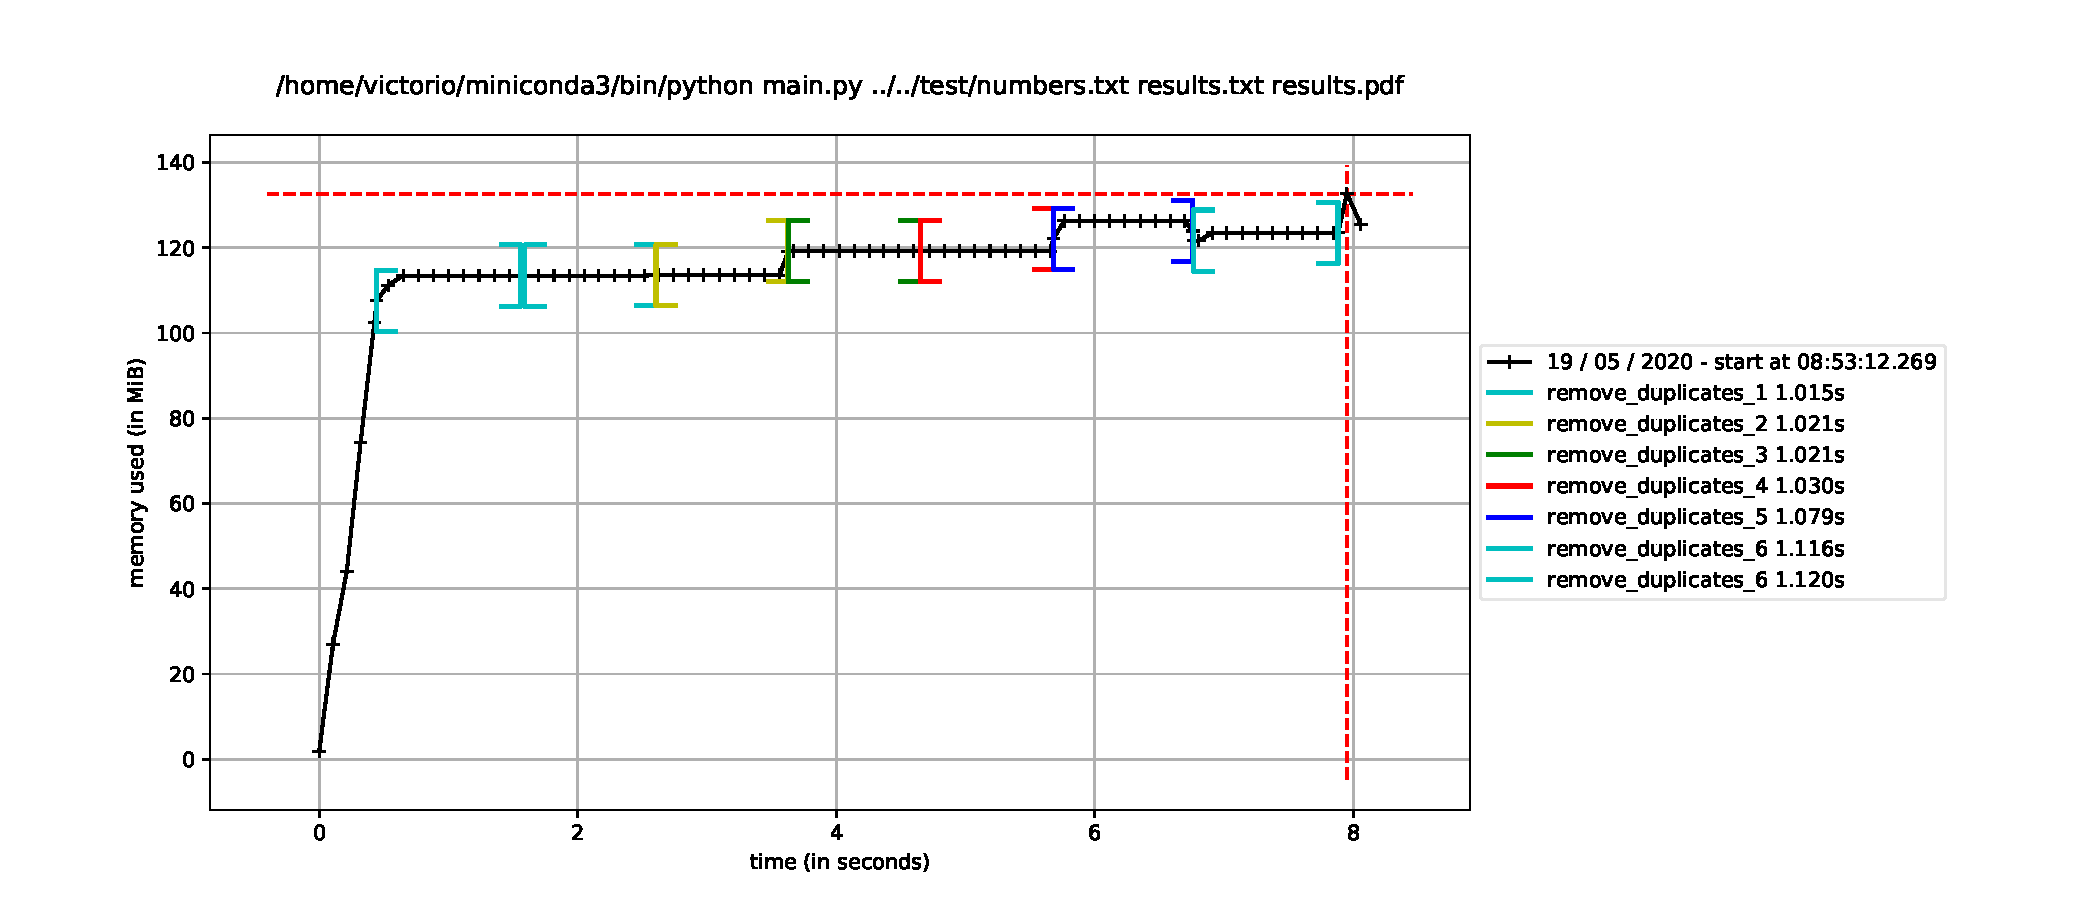
\includepdf[page=-]{memory_use_graph.pdf}

\subsubsection{Linear profiling y gráficas generadas con Matplotlib}
El profiling del tiempo de ejecución lo he realizado con el módulo \emph{linear\_profiling}, tal y como he comentado anteriormente. En el directorio \textbf{/doc/profiling} se puede encontrar su resultado, concretamente en el fichero \textbf{main.py.lprof}
Para terminar con el contraste de resultados, voy a incluir una serie de figuras (creadas con Matplotlib) compuestas por dos gráficos, uno de barras y otro de tarta, como ya comenté anteriormente.\\

Tal y como se comenta en el enunciado, el análisis lo he realizado, ademas de usando el módulo linear\_profiling, generando gráficas que muestran el tiempo usado por cada técnica para los distintos tamaños de datos, de 2000 en 2000, hasta llegar al tamaño total de la lista de elementos del fichero de entrada.\\

Pd: el siguiente contenido lo almacena el programa en el fichero correspondiente al tercer argumento que le pasa el usuario.\\

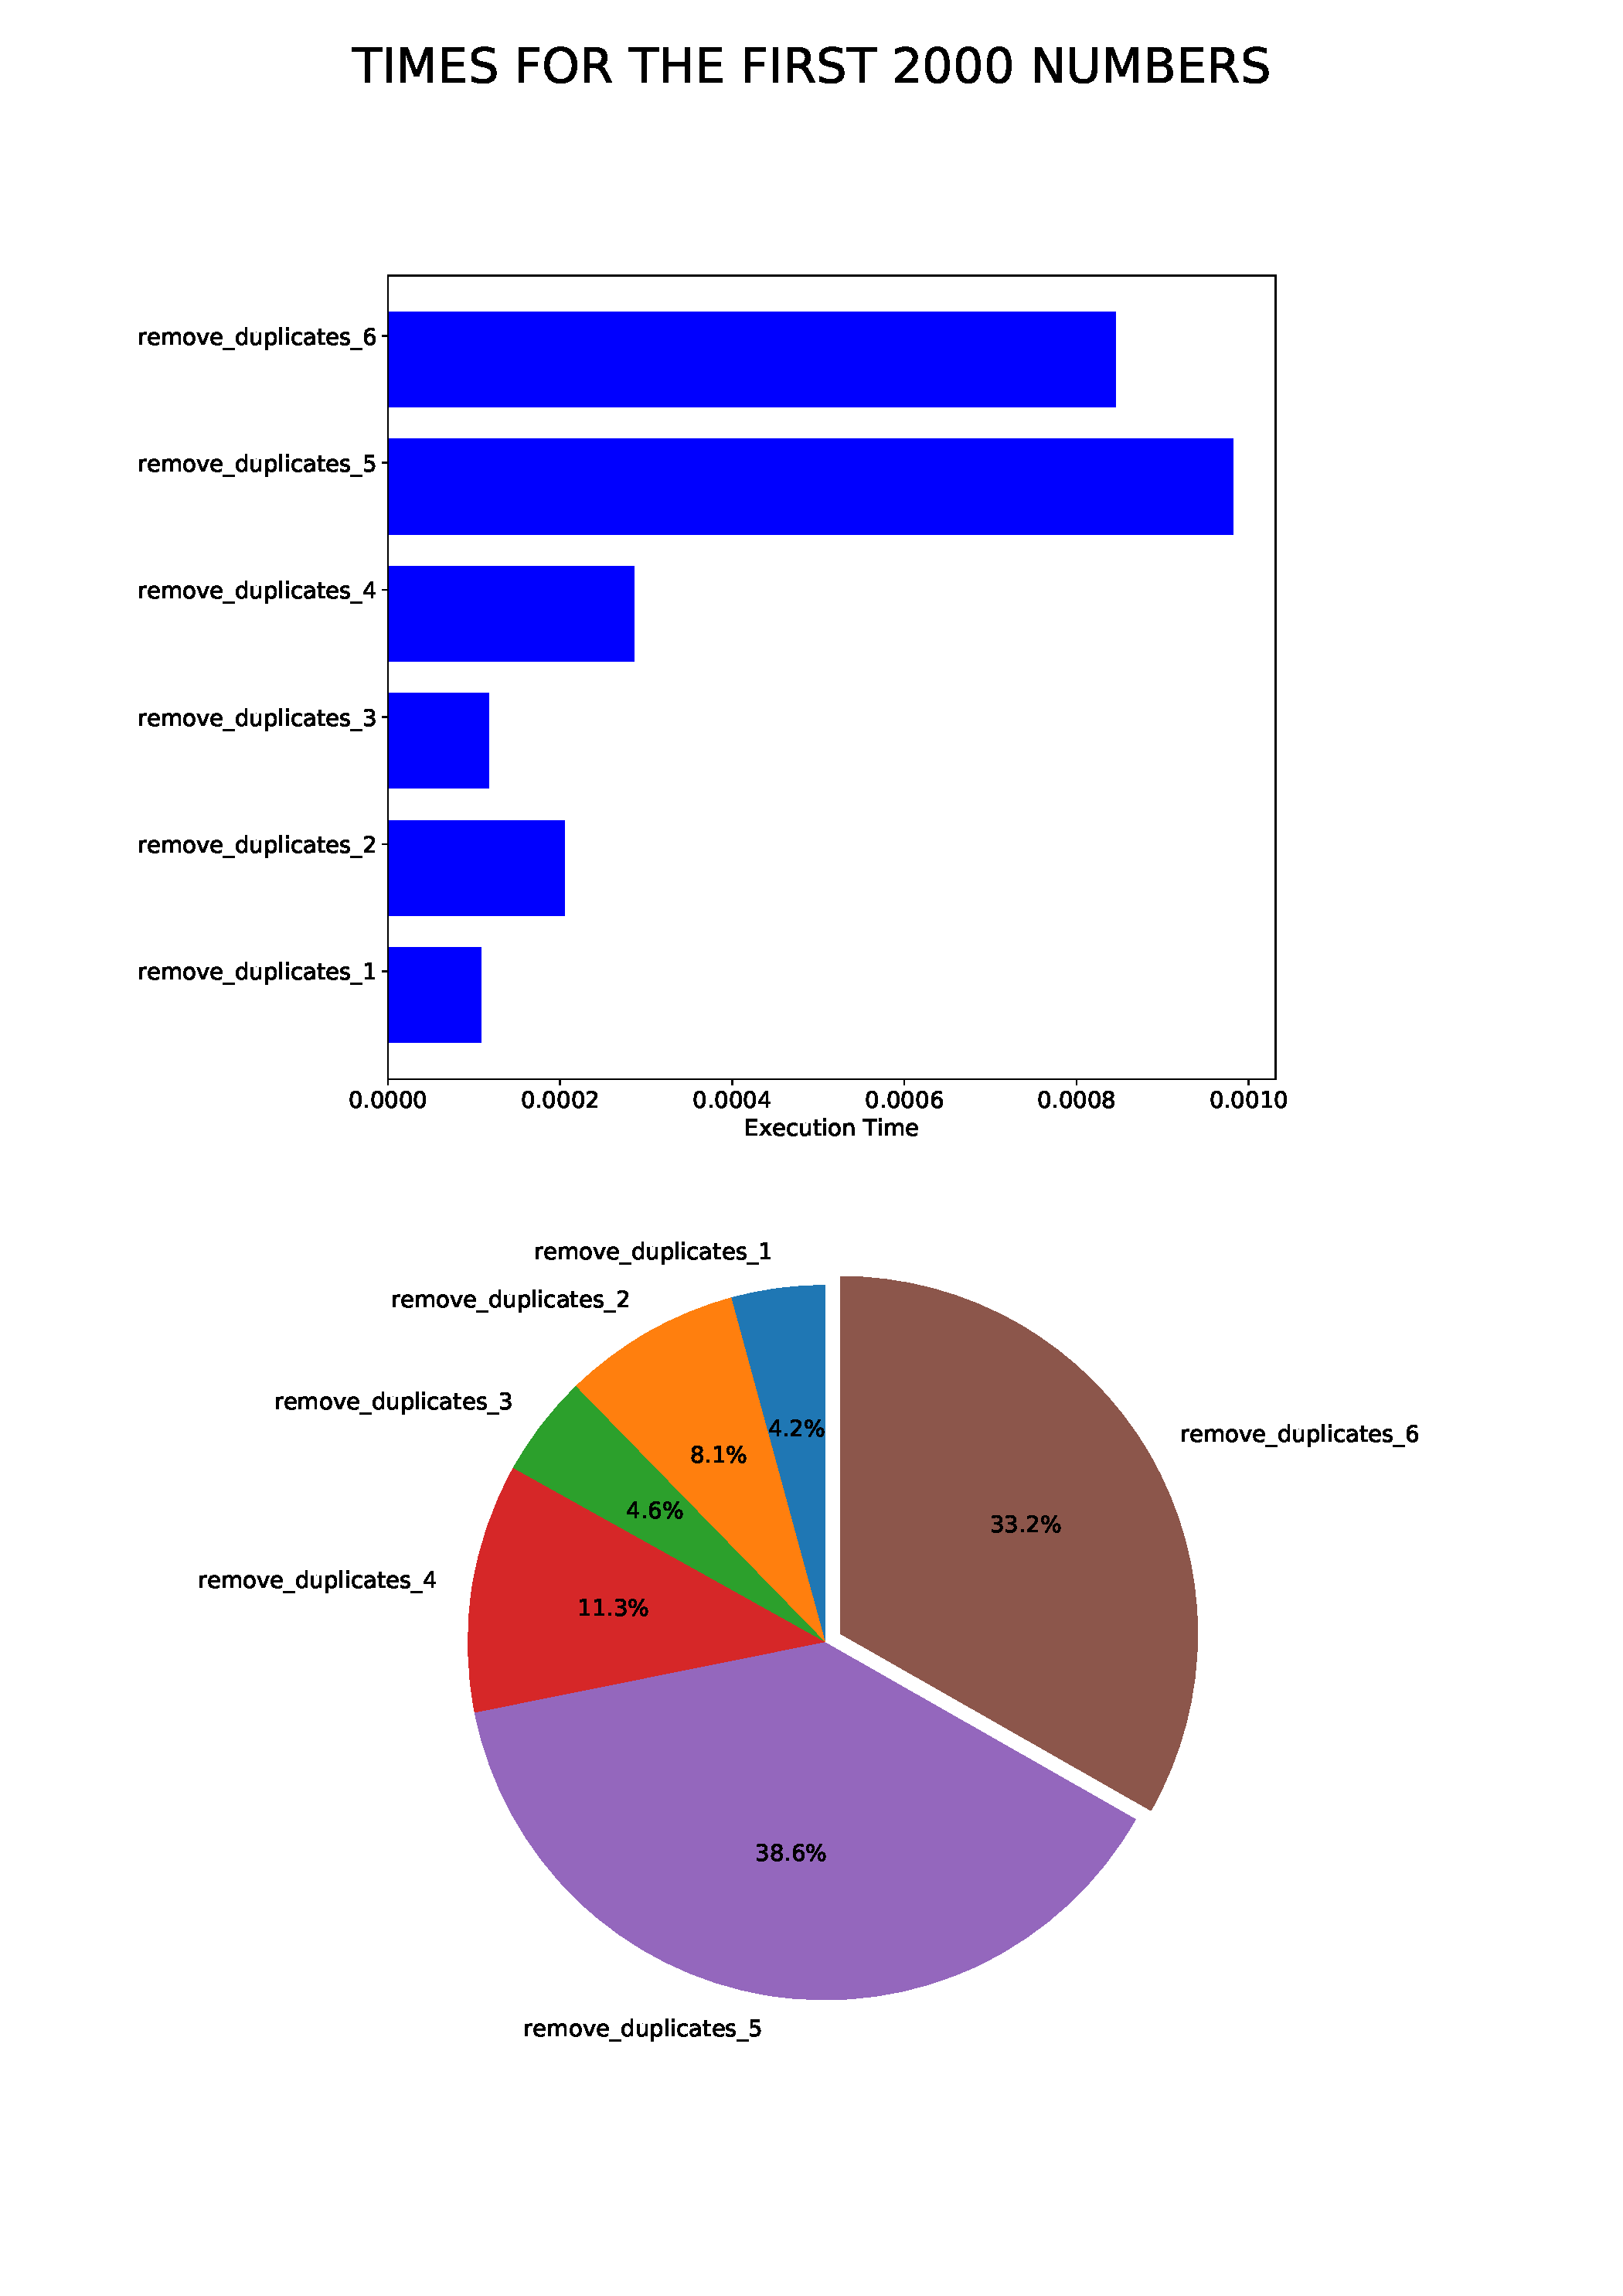
\includepdf[page=-]{execution_time_use_graph.pdf}

\section{Bibliografía}
\begin{thebibliography}{9}
\bibitem{latexcompanion} 
Michel Goossens, Frank Mittelbach, and Alexander Samarin. 
\textit{The \LaTeX\ Companion}. 
Addison-Wesley, Reading, Massachusetts, 1993.
\bibitem{einstein} 
Git.
\textit{Sobre el Control de Versiones}.
[\textit{Una breve historia de Git}]. 
\href{https://git-scm.com/book/es/v2/Inicio---Sobre-el-Control-de-Versiones-Una-breve-historia-de-Git}{https://git-scm.com/book/es/v2/Inicio---Sobre-el-Control-de-Versiones-Una-breve-historia-de-Git}
\bibitem{Profiling} 
Wikipedia
\textit{Análisis de rendimiento de software}.
\href{https://es.wikipedia.org/wiki/An%C3%A1lisis_de_rendimiento_de_software}{https://es.wikipedia.org/wiki/An\%C3\%A1lisis\_de\_rendimiento\_de\_software}
\bibitem{Matplotlib} 
Matplotlib
\textit{Generación de gráficos con Matplotlib}
\href{https://matplotlib.org/}{https://matplotlib.org/}
\end{thebibliography}
\end{document}

